\documentclass[11pt,dvipdfmx,b5paper,oneside]{jsbook}

\usepackage{graphicx}
\usepackage{color}
\usepackage{here}
\usepackage{framed}
\usepackage{tcolorbox}
\usepackage{quotchap}
\usepackage{pdfpages}
\usepackage[hidelinks]{hyperref}
\usepackage{pxjahyper}
\usepackage{titlesec}
\usepackage{picture}
\usepackage{tikz}

\usepackage{color}
\usepackage{xcolor}
\usepackage{listings}

\usepackage{caption}
\DeclareCaptionFont{white}{\color{white}}
\DeclareCaptionFormat{listing}{\colorbox{gray}{\parbox{\textwidth}{#1#2#3}}}

\captionsetup[lstlisting]{
 format=listing,
 singlelinecheck=true,
 labelfont=white,
 textfont=white
}
\lstset{
 backgroundcolor={\color[gray]{.85}},
 frame=shadowbox,
 numbers=left,
 tabsize=2
}
\renewcommand\lstlistingname{Code}

\tcbuselibrary{breakable}
\definecolor{shadecolor}{gray}{0.80}

% section
\titleformat{\section}[block]{}{}{0pt}
{
  \definecolor{teal}{gray}{0.30}
  \begin{picture}(0,0)
    \put(-10,-5){
      \begin{tikzpicture}
        \fill[teal] (0pt,0pt) rectangle (5pt,19pt);
      \end{tikzpicture}
    }
    \put(-10,-5){
      \color{teal}
      \line(1,0){\hsize}
    }
  \end{picture}
  \hspace{0pt}
  \sf \Large \thesection
  \hspace{0pt}
}

%\begin{tcolorbox}[breakable, title =test ]\label{asda}
%\begin{verbatim}
% using GR, PyPlot, Distributions
%\end{verbatim}
%\end{tcolorbox}
 
% 図表見出し
\renewcommand{\tablename}{\textcolor{gray}{▼} 表}
\renewcommand{\figurename}{\textcolor{gray}{▲} 図}

\begin{document}

\chapter{Data Visualization}
\section{Julia言語におけるデータの可視化}

Julia言語では、「Makie」,「Plots」などデータ可視化用のパッケージが提供されている。つぎ、「Makie」の特徴について説明しよう。Makieは、Juliaで作られた新しいパッケージである。またバイオリンプロットを始めとする高度な可視化ツールを含む。そのため、グラフの描写という目的においてMakieは強力なツールとなり得る。また、レイアウトの作成が簡単かつ細部まで技工を凝らすことが出来るというメリットがあり、科学論文に掲載する画像を作成するには最適だろう。次に「Plots」の特徴を説明しよう。「Plots」の特徴は、「PyPlot」や「GR」などの既成品のデータ可視化パッケージをバックエンドとして使用しグラフを描写する。つまり、「Plots」を使うことによって共通のコマンドで異なるパッケージを使用したデータの可視化を行うことが出来る。

そこで本章では、「Makie」,「Plots」の使用方法について説明する。もし、一つのパッケージ使用方法のみを習得したい場合は、「Makie」の学習を強くおすすめする。
\newpage


\section{Makieの使用方法について}
まず、Makieの使用方法の概要について説明しよう。Makieは、
\begin{enumerate}
 \item 軸ラベルなどの軸に関する描写を行う Axis layout
 \item 図の配置や図の大きさを構成する Figure layout
 \item 構成したFigure layout上に図を描写する関数
\end{enumerate}
の3要素を操作することによってグラフを作成することが出来る。このセクションでは、
図の書き方を説明した後、Axis layoutとFigure layoutの操作を説明する。

\subsection{Makieのインストール}
まず、Makieのインストールについて説明しよう。Makieは、デフォルトではVectorファイルのサポートがされていない。そこで、Vectorファイルの作成を可能とする「CairoMakie」を同時にインストールする必要がある。その他にも、HTMLに画像の埋め込みをするための「WGLMakie」があるので必要に応じてインストールを行う。それらのインストールは、下記のコマンド (Code. \ref{installMakie}) を実行することによって完了することが出来る。

\begin{lstlisting}[title =Makieのインストール, label=installMakie]
 using Pkg;
 Pkg.add("Makie")
 # vector ファイルを作成するために必要
 Pkg.add("CairoMakie")
 # HTMLに埋め込む場合
 # Pkg.add("WGLMakie")
\end{lstlisting}

\subsection{Makieを使用したグラフの描写}
この章では、
\begin{itemize}
 \item 一次元グラフ
 \begin{enumerate}
  \item ヒストグラム (histogram)
  \item カーネル密度推定 (kernel density plot)
  \item バイオリンプロット (violin plot)
  \item 棒グラフ (bar plot)
 \end{enumerate}
 \item 2次元グラフ
\begin{enumerate}
 \item 線グラフ (line plot)
 \item 散布図 (scatter plot)
 \item エラーバー (error bar plot)
 \item ベクトル図 (arrow plot)
 \item ヒートマップ (heatmap)
\end{enumerate}
\item 3次元グラフ
\begin{enumerate}
 \item ヒストグラム (histogram)
 \item メッシュプロット (mesh plot)
\end{enumerate}
\end{itemize}
の描写方法について説明する。また、使用可能なオプションに関しても適宜紹介する。

ここで、Makieを使用した基本的なグラフの描写方法について説明しよう。Makieを使用してグラフを書く際には、
\begin{description}
 \item{Step1. } 「Figure」関数を呼び出す
 \item{Step2. } 「Axis」関数を呼び出し、どの窓に描写するかを定義する
 \item{Step3. } どのAxisに描写するかを明示的に示した上でグラフを書く
\end{description}
の手続きを踏む。具体的な例として、$2\times2$のレイアウトのグラフの描写手続きについて説明しよう。
\begin{lstlisting}[title=Example]
  using CairoMakie, Makie
  # Figure 関数を呼び出す。
  # resolution = ( 縦の大きさ, 横の大きさ ) で画像の大きさを指定できる
  # backgroundcolor = 色  で背面の色を指定できる
  fig = Figure(resolution = (1200,1200), 
              backgroundcolor="gray"
              )
  # 使用するグラフの形状のレイアウトを決める
  # Axis を使用して Figure を分割する
  ax1 = Axis(fig[1,1]) bt6
  ax2 = Axis(fig[1,2])
  ax3 = Axis(fig[2,1:2])
  x = collect(1:0.1:10)
  scatter!(ax1, x, sin.(x)
  title )
  lines!(ax2, x, cos.(x) )
  scatter!(ax3, x, sin.(x) + cos.(x) )
  fig
\end{lstlisting}
こんな感じで、書く。

\begin{figure}[h]
  \centering
  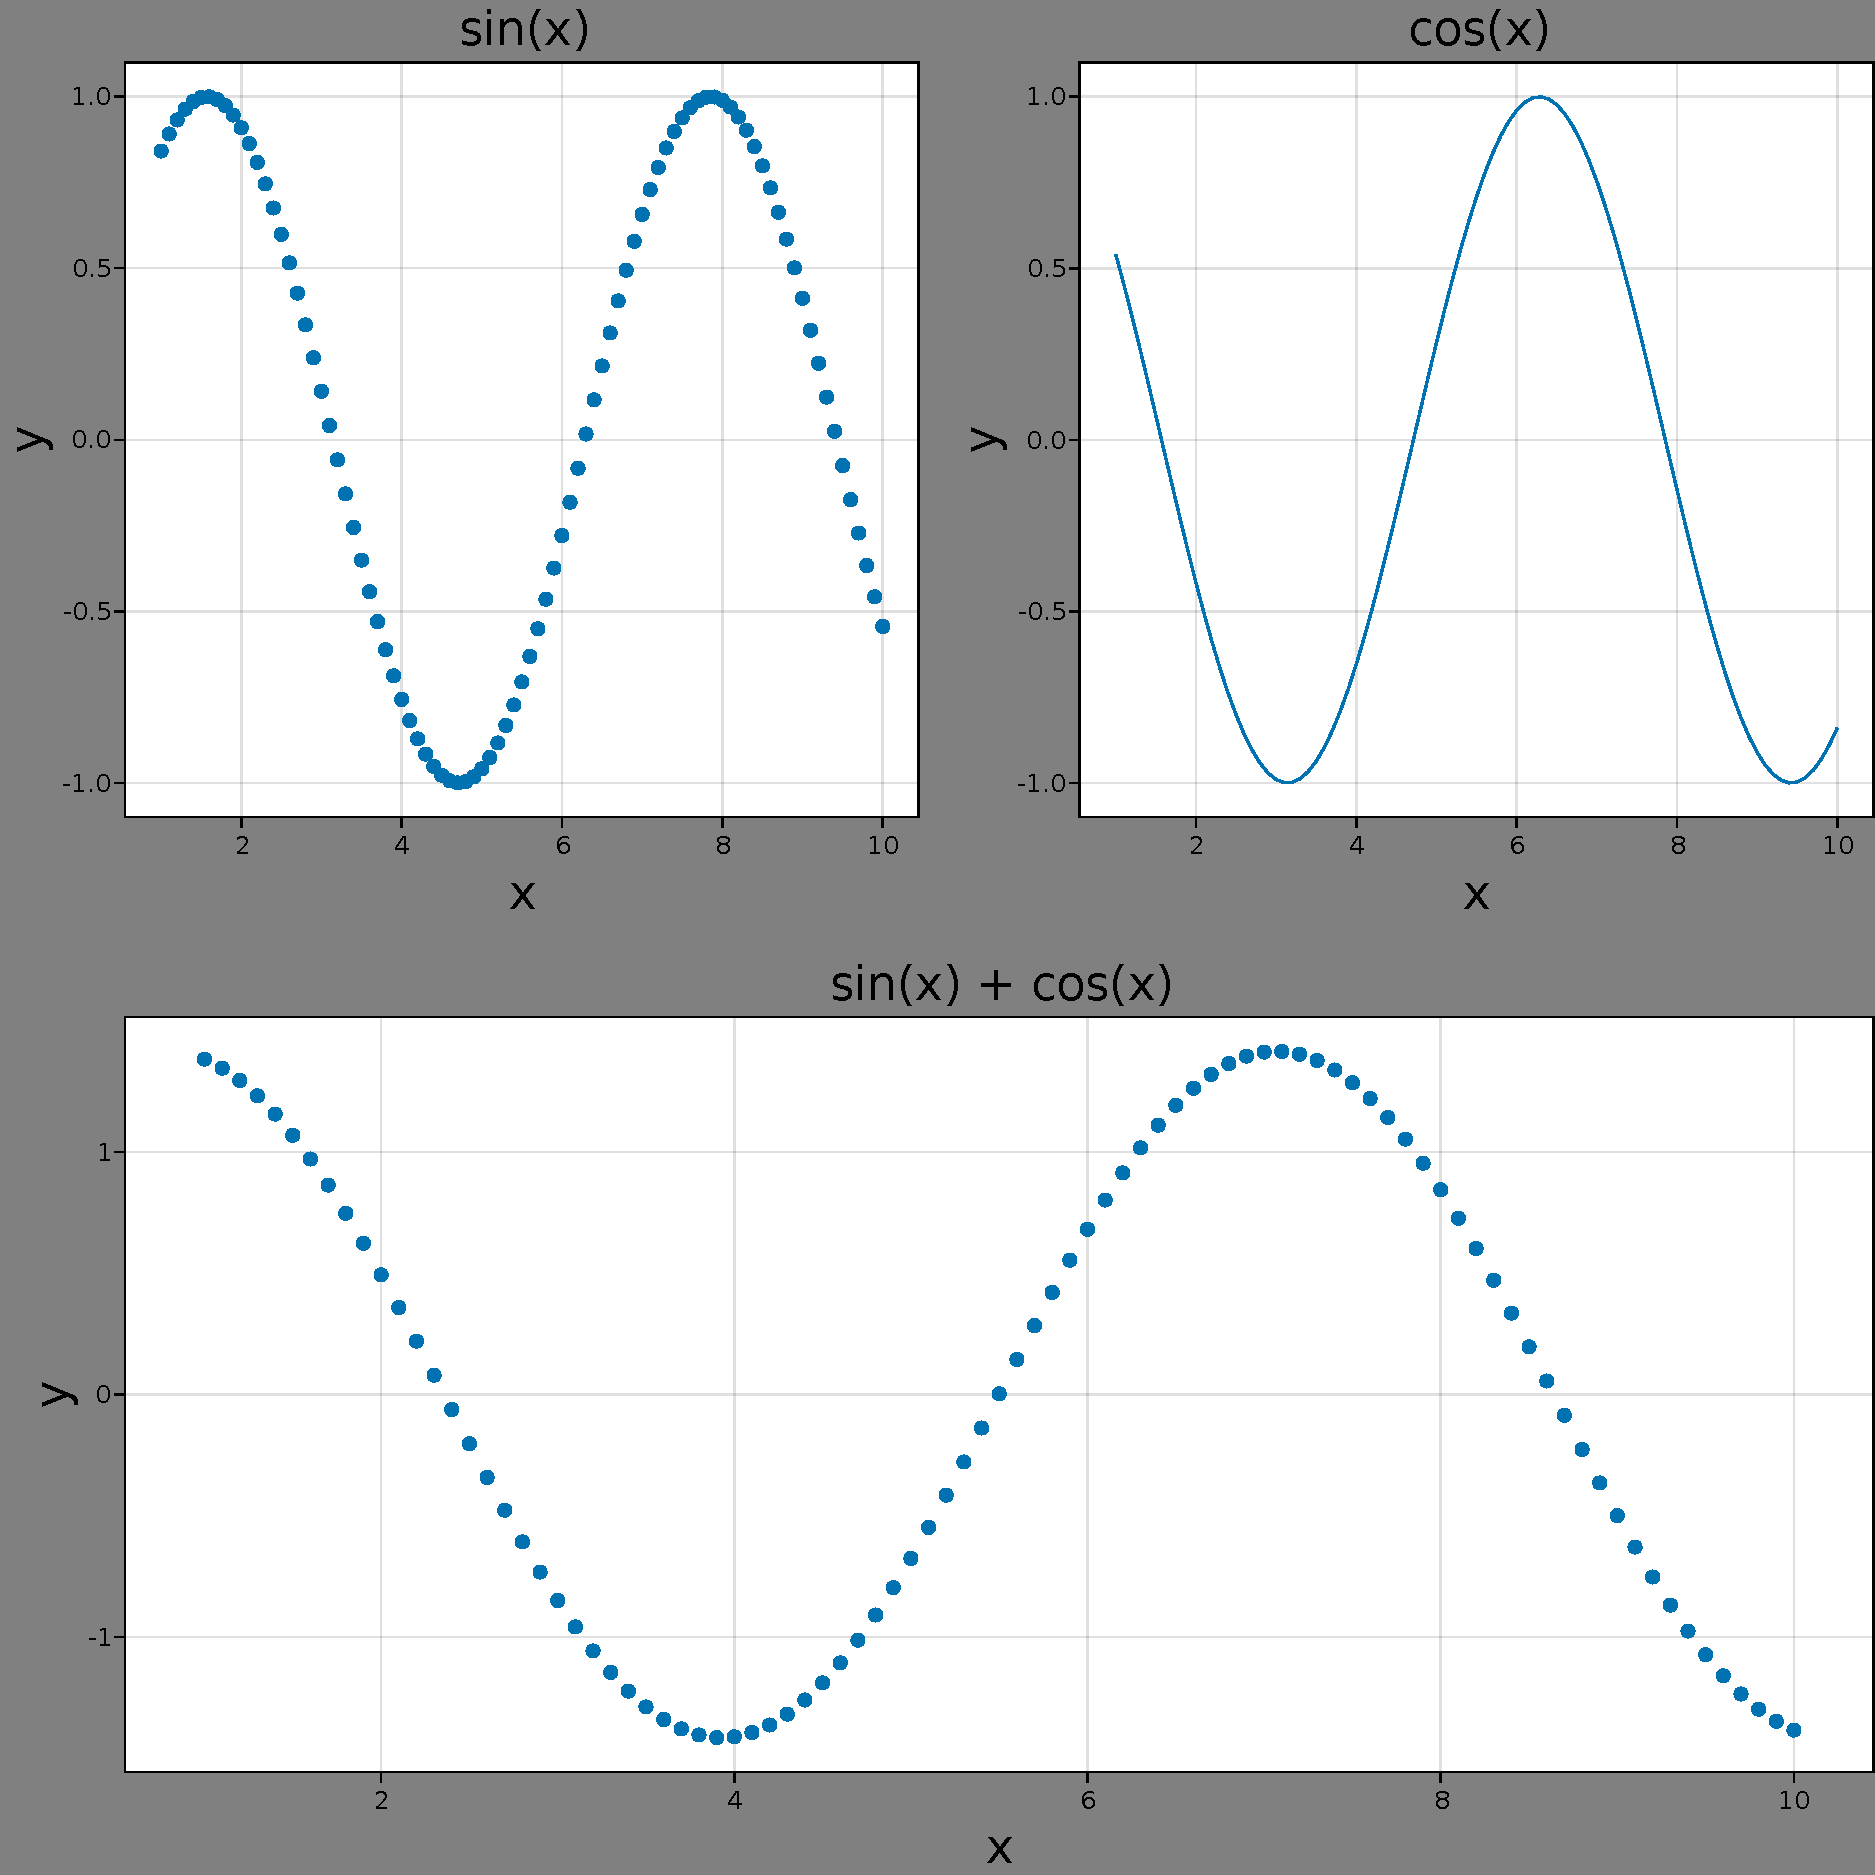
\includegraphics[keepaspectratio, width=12cm, height=12cm]{example1.pdf}
 \end{figure}

\subsection{1次元グラフ}
データ分析を行う際には各変数の定性的な性質を分析することが重要である。例えば、分布関数の形状や条件付き分布などが統計量の定性的な性質を示す統計量である。これらの統計的な定性的な性質を調べることは、理論モデルの発展や適切な統計分析を行う上で重要である。

まず、分布関数の定性的な性質を描写するヒストグラムの描写方法について説明しよう。ここでは、サンプルデータとしてirisデータセットを使用する。



\subsubsection{2次元グラフ}
線グラフは、独立変数である$x$と従属変数である$y$に明確な関係がある時に有効な可視化手法である。例えば、観測されるデータに $y = x^2$という関係式が期待される場合を考えよう。
\newpage
\section{Plots}

ここで、Plotsについて紹介しよう。まず、Plotsの特徴である「共通のコマンド使用しグラフを描写」を説明するために「PyPlot」と「GR」を使用したヒストグラムのコード (Code \ref{gr_pyplot_compare}) を比較しよう。
\begin{lstlisting}[label=gr_pyplot_compare ,caption=PyPlotとGRを使用したヒストグラムの描写]
using GR, PyPlot
plt = PyPlot
gr = GR
# PyPlot
x = randn(1000)
plt.hist(x)
plt.xlabel("counts")
plt.savefig("hist_pyplot.pdf")
plt.show()
# GR
gr.histogram(x)
gr.xlabel("counts")
gr.savefig("hist_gr.pdf")
\end{lstlisting}

\begin{figure}
 \begin{minipage}[b]{0.45\linewidth}
   \centering
   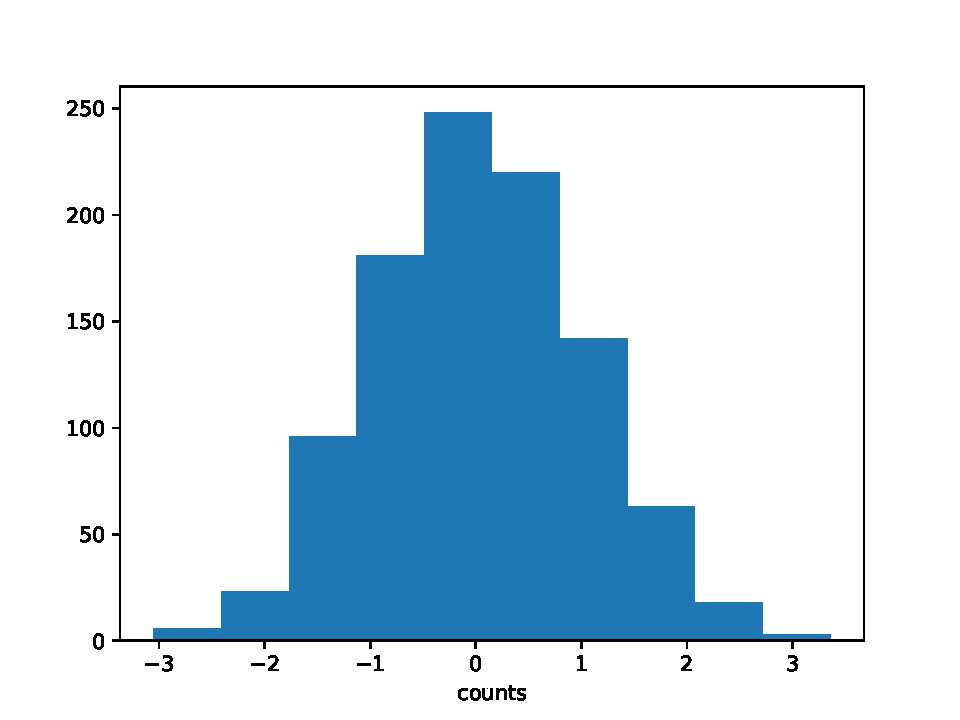
\includegraphics[keepaspectratio, width=5cm, height=5cm]{hist_pyplot.pdf}
 \end{minipage}
 \begin{minipage}[b]{0.45\linewidth}
   \centering
   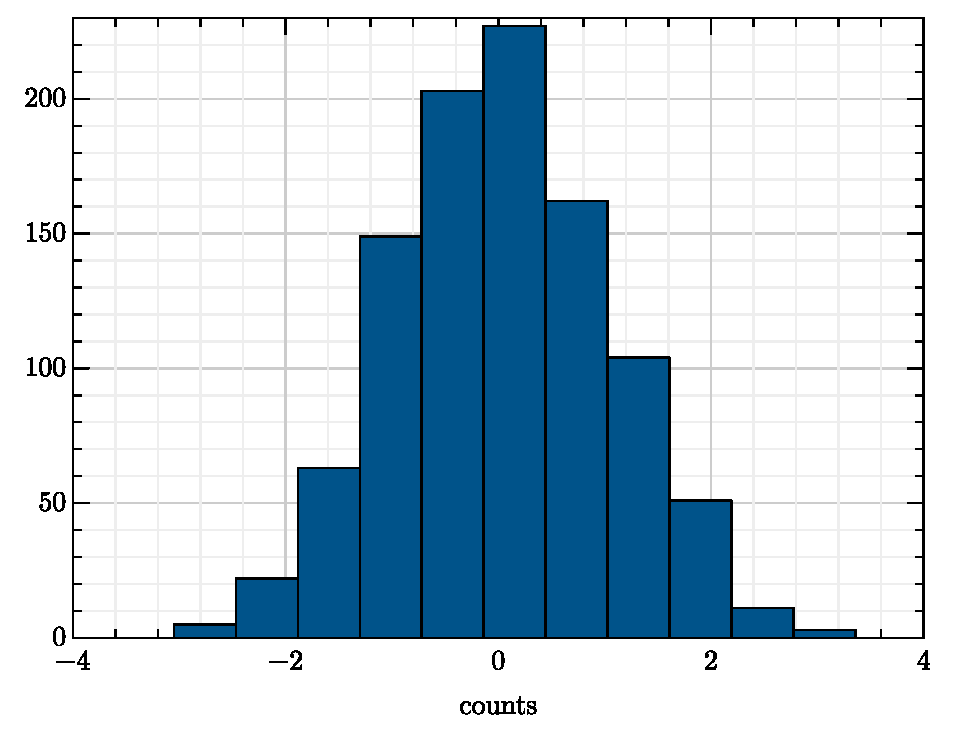
\includegraphics[keepaspectratio, width=5cm, height=5cm]{hist_gr.pdf}
 \end{minipage}
 \caption{左:PyPlotsを使用したhistogramの描写。右:GRを使用したhistogramの描写}
\end{figure}
このようにしてヒストグラムを生成できるのだが、「PyPlot」では「hist」、「GR」では「histogram」のように使用する関数名が異なる。この差は異なるパッケージを使用する時に、エラー発生確率の上昇 (GRを使用している時にPyPlotのコマンドを誤って使用する) のような形で現れると期待される。そのため、関数名が揃っていることは重要である。

\section{Makie}
\begin{shaded}
\begin{verbatim}
## ここにはコマンドを書く
$ echo "Hello, World!"
\end{verbatim}
\end{shaded}

図表はキャプションを付けたときに、先頭に「▲」や「▼」を付けるようにした。

\begin{table}[H]
  \centering
  \caption{表のサンプル}
  \begin{tabular}{|c|l|l|l|} \hline
    日本 & hoge & fuga & piyo \\ \hline
    アメリカ & foo & bar & baz \\ \hline
  \end{tabular}
  \label{table-sample}
\end{table}

%\begin{figure}[H]
%  \centering
%  \includegraphics[width=4cm]{sample.jpg}
%  \caption{画像のサンプル}
%  \label{figure-sample}
%\end{figure}

\begin{tcolorbox}[title=これはコラム]
  コラムも随時挟めるようにした。

  tcolorboxはtitleを指定するといい感じにタイトル付きの枠で囲ってくれる。
\end{tcolorbox}

\end{document}